\documentclass[letter,graphicx]{beamer}



\mode<presentation>
{
  \usetheme{Warsaw}
  % or ...

  \setbeamercovered{transparent}
  % or whatever (possibly just delete it)
}


\usepackage[english]{babel}
% or whatever

\usepackage[latin1]{inputenc}
% or whatever
\usepackage{verbatim}
\usepackage{times}
\usepackage[T1]{fontenc}
% Or whatever. Note that the encoding and the font should match. If T1
% does not look nice, try deleting the line with the fontenc.

\logo{}
%\logo{
\includegraphics[width=.1\textwidth]{./images/official_NOAA_logo.pdf}}

\title[Bayes, MCMC, and genotyping errors] % (optional, use only with long paper titles)
{Bayesian Inference, MCMC, and \\
Genotyping Error
}

\subtitle{} % (optional)

\author[Eric C. Anderson] % (optional, use only with lots of authors)
{Eric C.~Anderson}
% - Use the \inst{?} command only if the authors have different
%   affiliation.

\institute[NOAA Fisheries] % (optional, but mostly needed)
{\mbox{}
Fisheries Ecology Division, Southwest Fisheries Science Center, Santa Cruz
\hfill
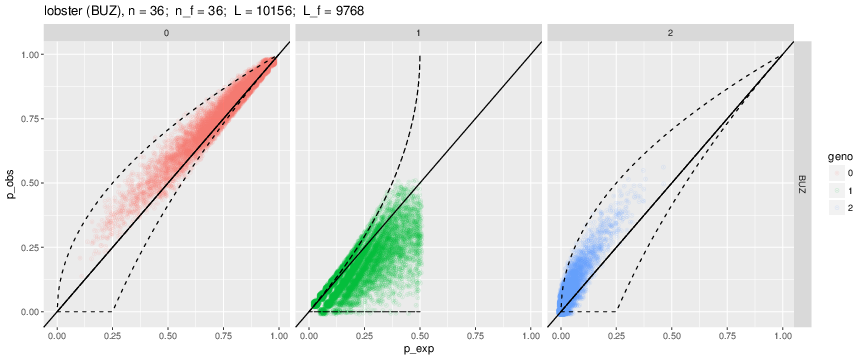
\includegraphics[height=.25\textwidth]{./images/lobster_big_pop.png}
\hfill
}
% - Use the \inst command only if there are several affiliations.
% - Keep it simple, no one is interested in your street address.

\date[BAPG 2018] % (optional)
{
ConGen 2018, Flathead Lake Biological Station \\ 10 SEPT 2018}

\subject{Talks}


\newcommand{\thh}{^\mathrm{th}}
\newcommand{\tc}{\textcolor}
\def\bm#1{\mathpalette\bmstyle{#1}}
\def\bmstyle#1#2{\mbox{\boldmath$#1#2$}}
\newcommand{\bY}{\bm{Y}}


\begin{document}




\begin{frame}
  \titlepage
\end{frame}





\begin{frame}{Overview}


\begin{itemize}
\item Models and MCMC
    \begin{itemize}
    \item Estimating allele frequencies
    \item Brief overview of MCMC by way of visualization
    \item Add a layer to the model (genotypes)
    \item Component-wise MCMC / Gibbs Sampling
    \end{itemize}
\item Assessing genotyping errors
    \begin{itemize}
    \item Genotype frequency visualizations
    \item A model for heterozygote miscall rate
    \item Add read depths to the model
    \item Hands-on session
    \end{itemize}

\end{itemize}
\end{frame}




\begin{frame}{A DAG for Allele Frequency Probabilities}

\begin{center}
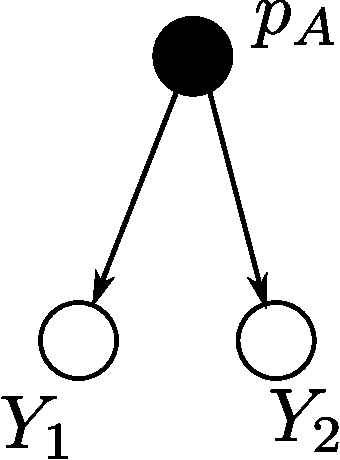
\includegraphics[height=.30\textheight]{../diagrams/slide_simple1-crop.pdf}
\end{center}
\begin{itemize}
\item Relationships in graph express factorization as conditional probabilities.
\item The above assumes Hardy-Weinberg conditions
\end{itemize}
$$
\small
P(\mbox{Individual is AA}~|~p_A) = P(Y_1 = A~|~p_A) P(Y_2 = A~|~p_A) = p_A \cdot p_A =  p_A^2
$$
\end{frame}





\begin{frame}{}
\begin{center}
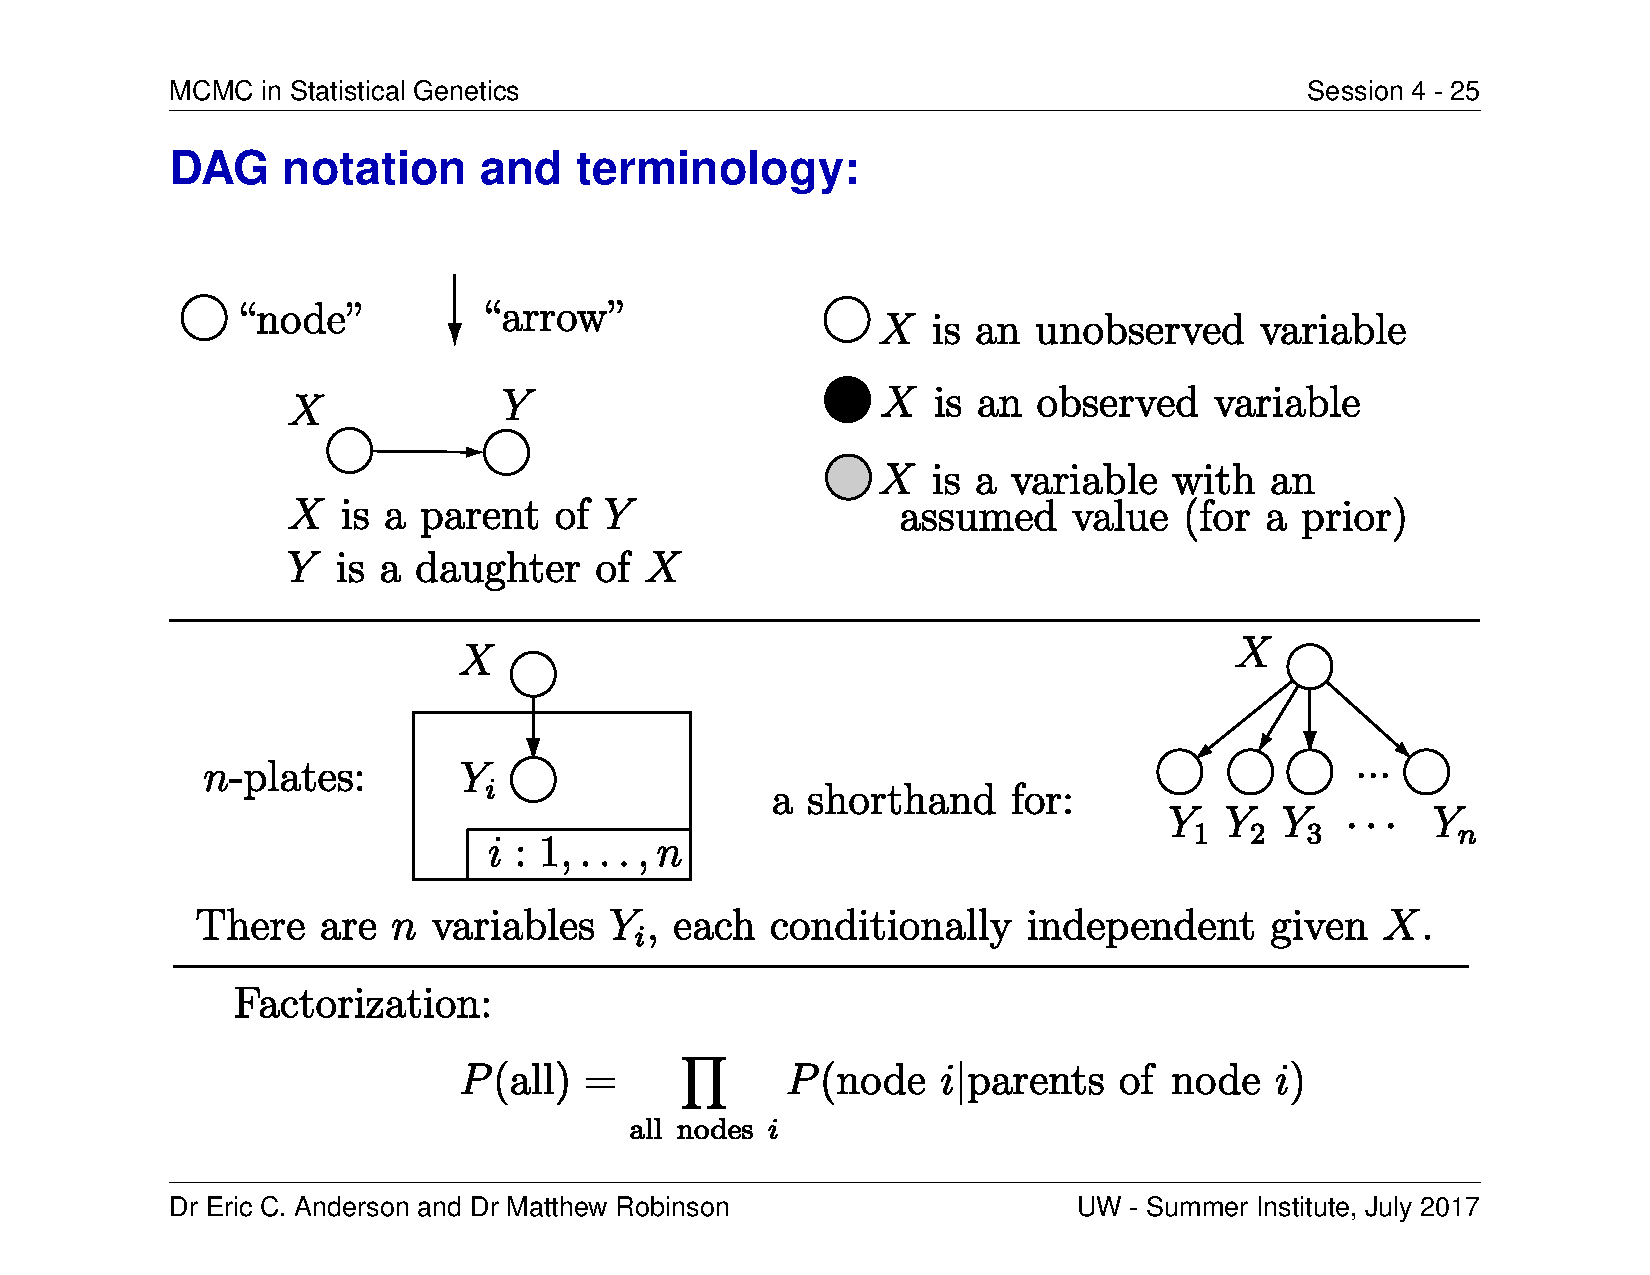
\includegraphics[width=.95\textwidth]{../slide_grabs/dag-notes.pdf}
\end{center}
\end{frame}





\begin{frame}{Estimating Allele Freqs from a Sample}
\framesubtitle{This depicts a sample of $N$ diploids}
\begin{center}
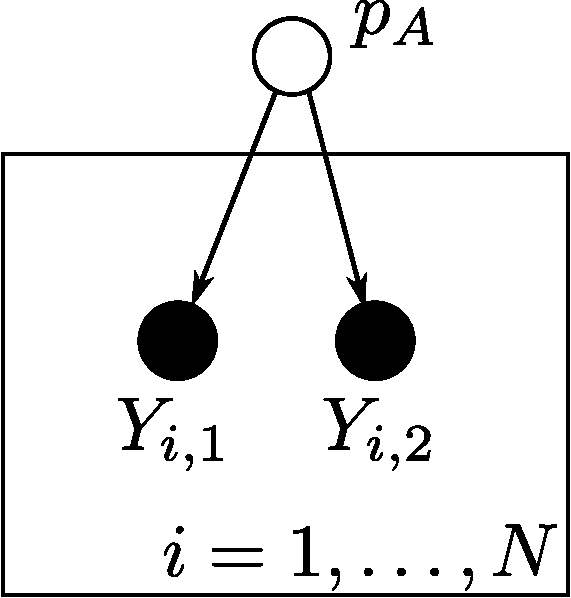
\includegraphics[height=.65\textheight]{../diagrams/slide_infer1-crop.pdf}
\end{center}
\begin{itemize}
\item To be Bayesian about this we must update our prior beliefs about $p_A$, using our data.
\end{itemize}
\end{frame}






\begin{frame}{A DAG for Bayesian Inference}
\framesubtitle{You have to assume a prior}
\begin{columns}
    \begin{column}{0.31\textwidth}
        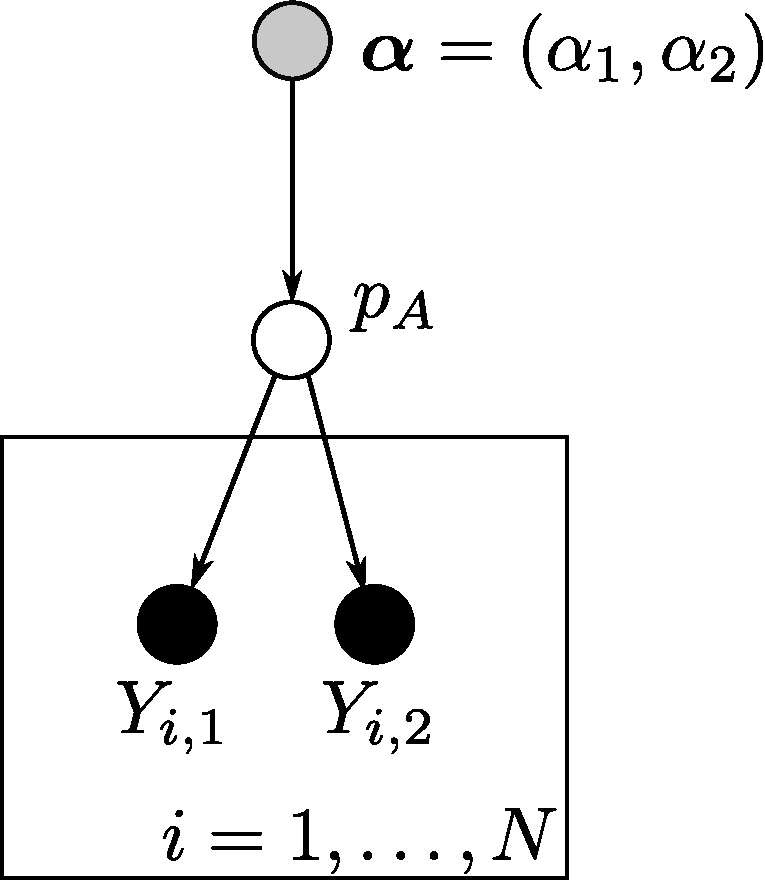
\includegraphics[width=1.0\textwidth]{../diagrams/slide_infer1-with-prior-crop.pdf}
    \end{column}
    \begin{column}{0.69\textwidth}
    	\begin{itemize}
		\item The DAG shows:
        \begin{itemize}
        \item $\bm{\alpha}$~~~~the parameters of the (beta) prior for allele frequencies
        \item $p_A$~~~~unknown frequency of allele $A$ at the locus
        \item $Y_{i,1}, Y_{i,2}$~~~~the observed (called/scored) alleles at diploid individual $i$
        \end{itemize}
        \item Bayesian inference means finding the {\em posterior distribution} for $p_A$.
        \begin{itemize}
        \item \mbox{$P(p_A|\bY) \propto P(p_A,\bY) = P(p_A|\bm{\alpha}) P(\bY|p_A)$}
        \end{itemize}
        \end{itemize}
    \end{column}
\end{columns}
\end{frame}














\begin{frame}{The Beta Distribution}
\framesubtitle{The standard prior for allele frequencies}

\begin{center}
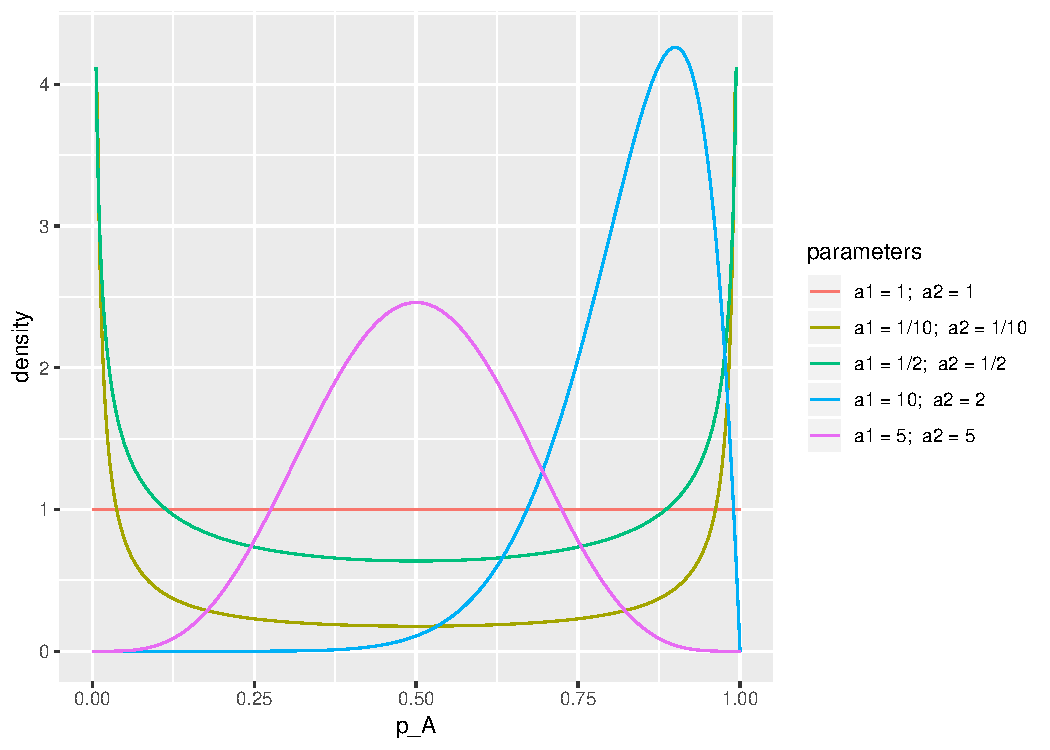
\includegraphics[width=.75\textwidth]{../figures/beta_densities.pdf}
\end{center}
\begin{itemize}
\item Very flexible family of distributions
\item Conjugate prior for binomial data
\end{itemize}
\end{frame}





\begin{frame}{Our updated or {\em posterior} distribution}
\framesubtitle{In this case it can be obtained analytically}
\begin{center}
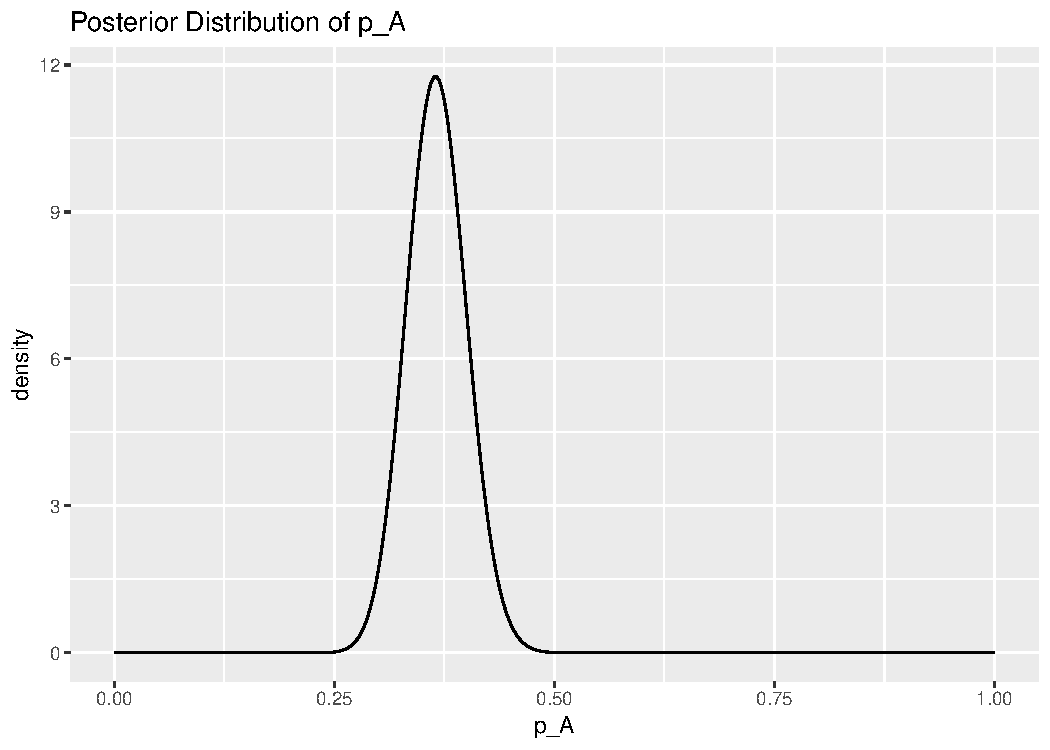
\includegraphics[height=.55\textheight]{../figures/pa_posterior.pdf}
\end{center}
\begin{itemize}
\item Imagine $N=100$ so we have $2N=200$ and we see 73 copies of the $A$ allele. 
\item Sample proportion = $73/200 \approx 0.37$.
\item \fbox{Computer Demos about Monte Carlo sampling}
\end{itemize}
\end{frame}








\begin{frame}{A DAG for probabilistic genotype calling}

\begin{center}
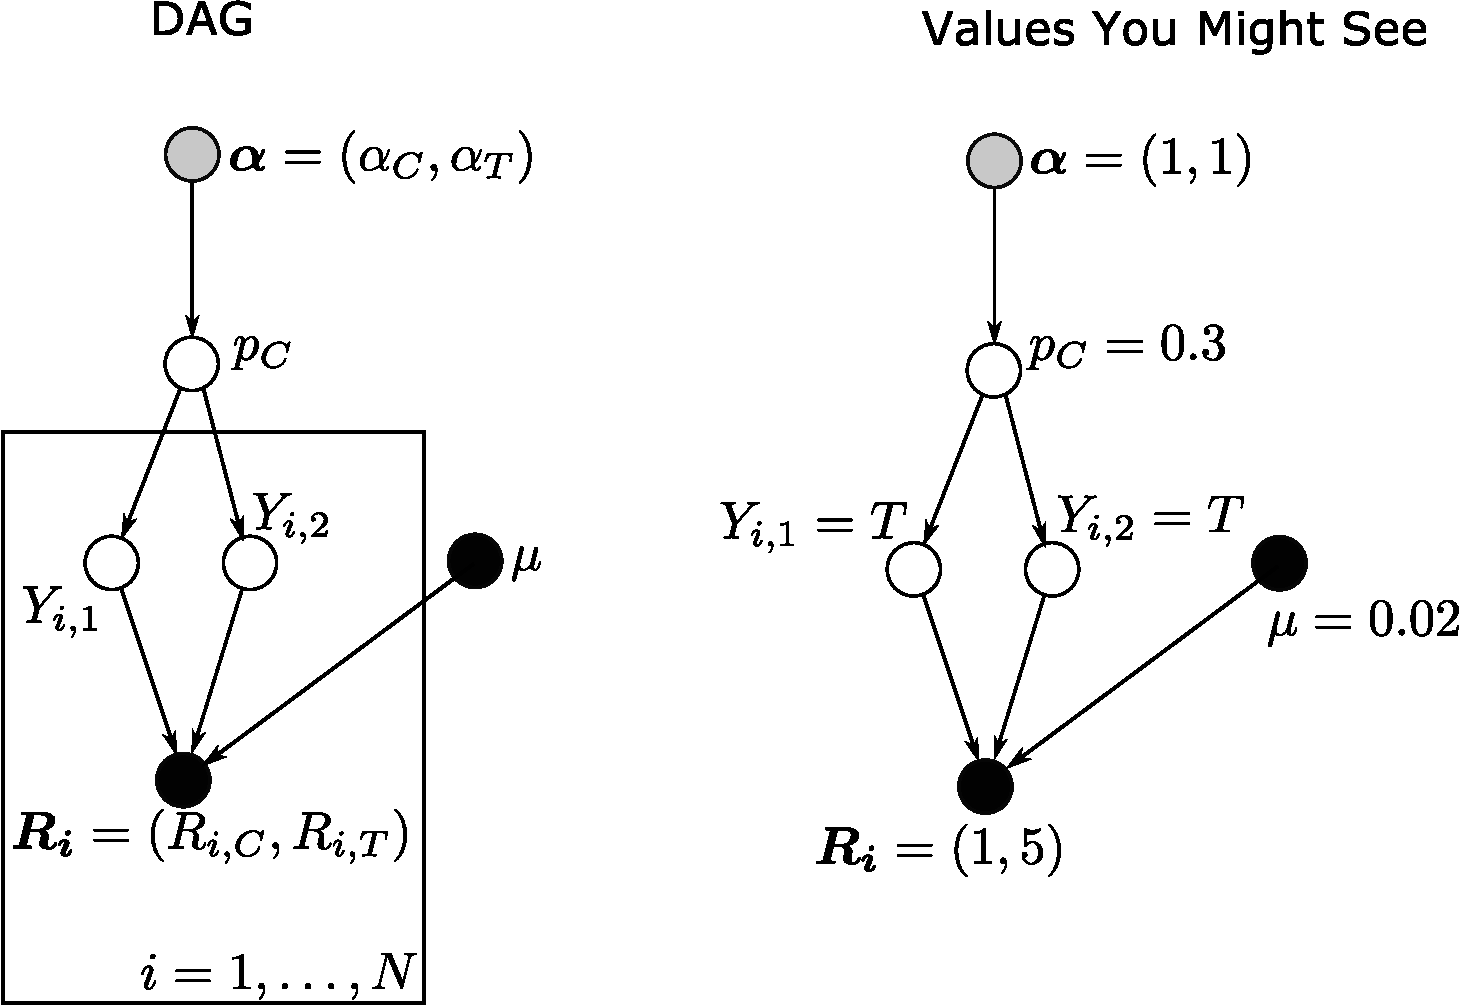
\includegraphics[width=.65\textwidth]{../diagrams/slide_genos-and-reads-dag-crop.pdf}
\end{center}
\begin{itemize}
\item $Y_{i,1}$ and $Y_{i,2}$: the true genotype of the $i\thh$ individual (now considered unobserved or {\em latent})
\item $(R_{i,C}, R_{i,T})$ number of reads covering the SNP with either a $C$ or a $T$.
\item $\mu$: rate of sequencing error
\end{itemize}
\end{frame}








\begin{frame}{Gibbs Sampling}
\framesubtitle{A type of {\em component-wise} MCMC}
The recipe for Gibbs sampling
\begin{itemize}
\item Start with some initial (often random) values for all the latent variables and parameters
\item At each step, choose a subset of the variables, and simulate new values for that subet
conditional on all the remaining ones.
\end{itemize}
To give an intuitive, visual understanding of this we shall digress for a few slides to
consider the hierarchical model underlying the program {\em structure}.
\end{frame}



\begin{frame}{Conceptual Model Underlying {\em structure}~---~I}

\begin{center}
\includegraphics*[width=.75\textwidth]{../figures/admixture_cats.pdf}
\end{center}
\end{frame}






\begin{frame}{Conceptual Model Underlying {\em structure}~---~II}
\begin{center}
\includegraphics*[width=\textwidth]{../figures/admix_cat_flags.pdf}
\end{center}
\end{frame}




\begin{frame}{The DAG for the {\em structure} model}
\begin{columns}
    \begin{column}{0.41\textwidth}
        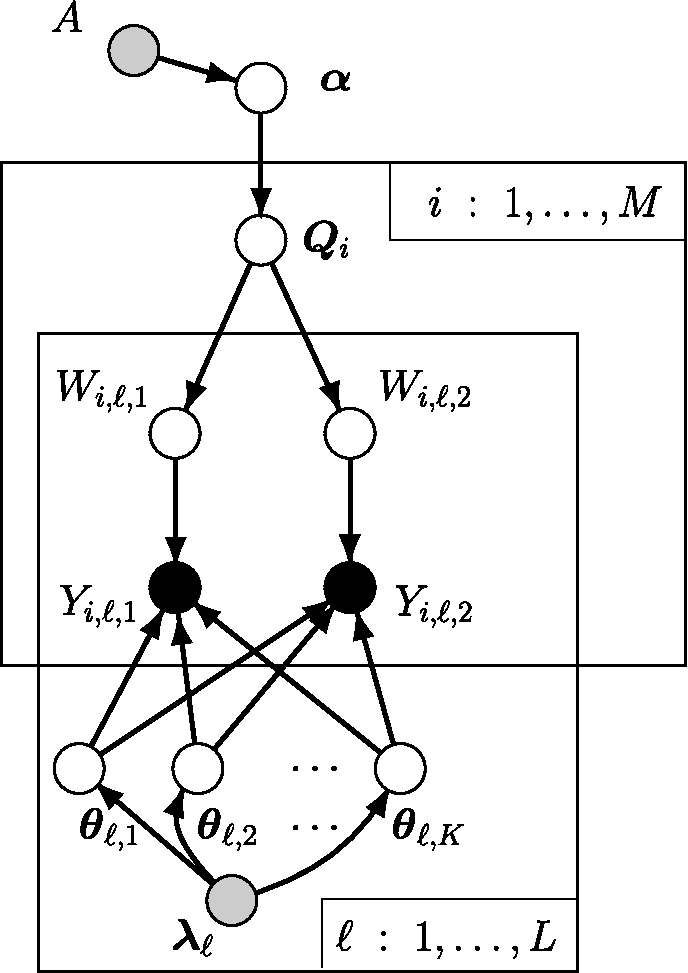
\includegraphics[width=1.0\textwidth]{../diagrams/PritchSimple.pdf}
    \end{column}
    \begin{column}{0.59\textwidth}
    	\begin{itemize}
		\item $A$~:~maximum possible value for each $\alpha_k$.
		\item $\bm{\alpha}$~:~parameters of the prior on ancestry proportions
		\item $\bm{Q}_i$~:~ancestry proportions of individual $i$
		\item $W_{i,\ell,1}$, $W_{i,\ell,2}$~:~``gene pool'' of origin of the two 
		gene copies at the $\ell\thh$ locus in the $i\th$ individual. 
		\item $Y_{i,\ell,1}$, $Y_{\i,\ell,1}$~:~allelic type of the two gene
		copies at locus $\ell$ in indiv $i$.
		\item $\bm{\theta}_{\ell,k}$~:~allele frequencies at locus $\ell$ in ``gene pool'' $k$.
        \end{itemize}
    \end{column}
\end{columns}
\end{frame}



\begin{frame}{Gibbs Sampling in the {\em structure} model~---~I}
\framesubtitle{Initialization}
\begin{columns}
    \begin{column}{0.41\textwidth}
        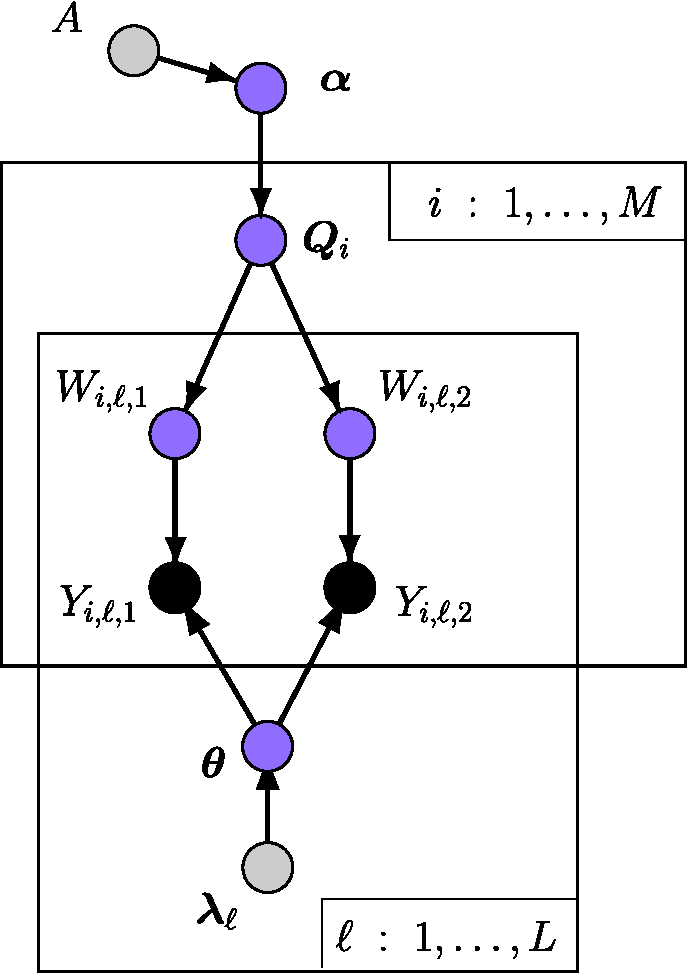
\includegraphics[width=1.0\textwidth]{../diagrams/PritchSimple2_purp.pdf}
    \end{column}
    \begin{column}{0.59\textwidth}
    	\begin{itemize}
		\item Pretend that you knew the values of all the latent variables (shaded purple here) which we will collectively call $\mathbf{X} = (\bm{\alpha}, \bm{Q},\mathbf{W}, \bm{\theta})$.
		\item AND
		\item the value of these latent variables was randomly drawn
		from their conditional distribution given $\mathbf{Y}$ and the priors.
        \end{itemize}
    \end{column}
\end{columns}
\end{frame}



\begin{frame}{Gibbs Sampling in the {\em structure} model~---~II}
\framesubtitle{Update variables in turn}
\begin{columns}
    \begin{column}{0.41\textwidth}
        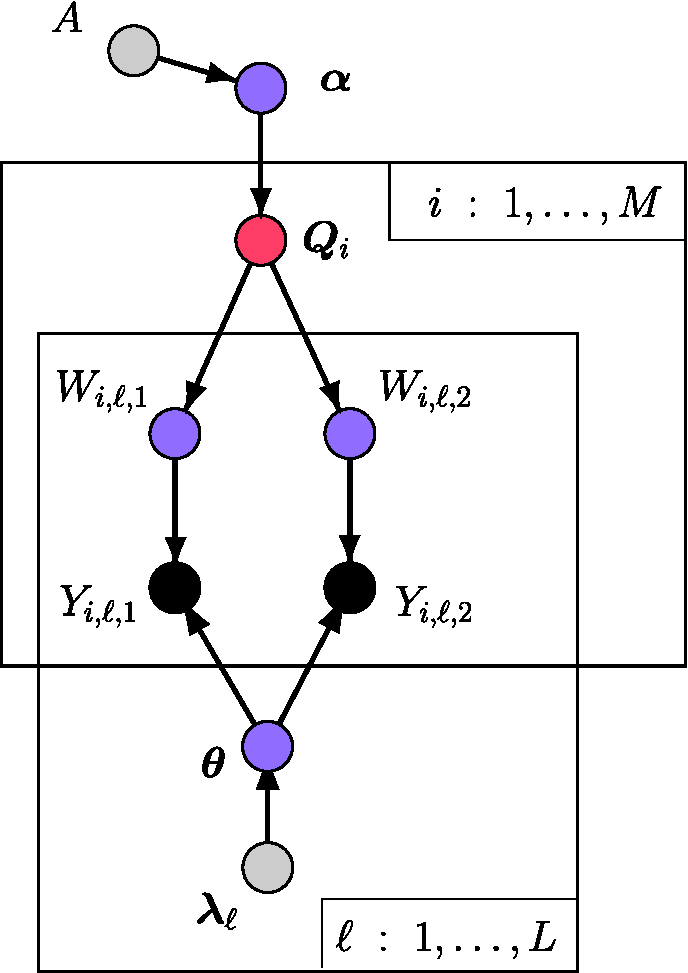
\includegraphics[width=1.0\textwidth]{../diagrams/PritchSimple2_purpQprime.pdf}
    \end{column}
    \begin{column}{0.59\textwidth}
    	\begin{itemize}
		\item Focus just on the $\bm{Q}_i$ for one individual $i$, and simulate a 
		new value from it's full conditional distribution.
		\item Do that for every individual $i$.
		\item Then do the same thing for the allele frequencies,
		\item and then for the $W$'s\ldots
		\item \fbox{Computer Demo}
        \end{itemize}
    \end{column}
\end{columns}
\end{frame}






\begin{frame}{Back to probabilistic genotype calling}
\begin{columns}
    \begin{column}{0.31\textwidth}
        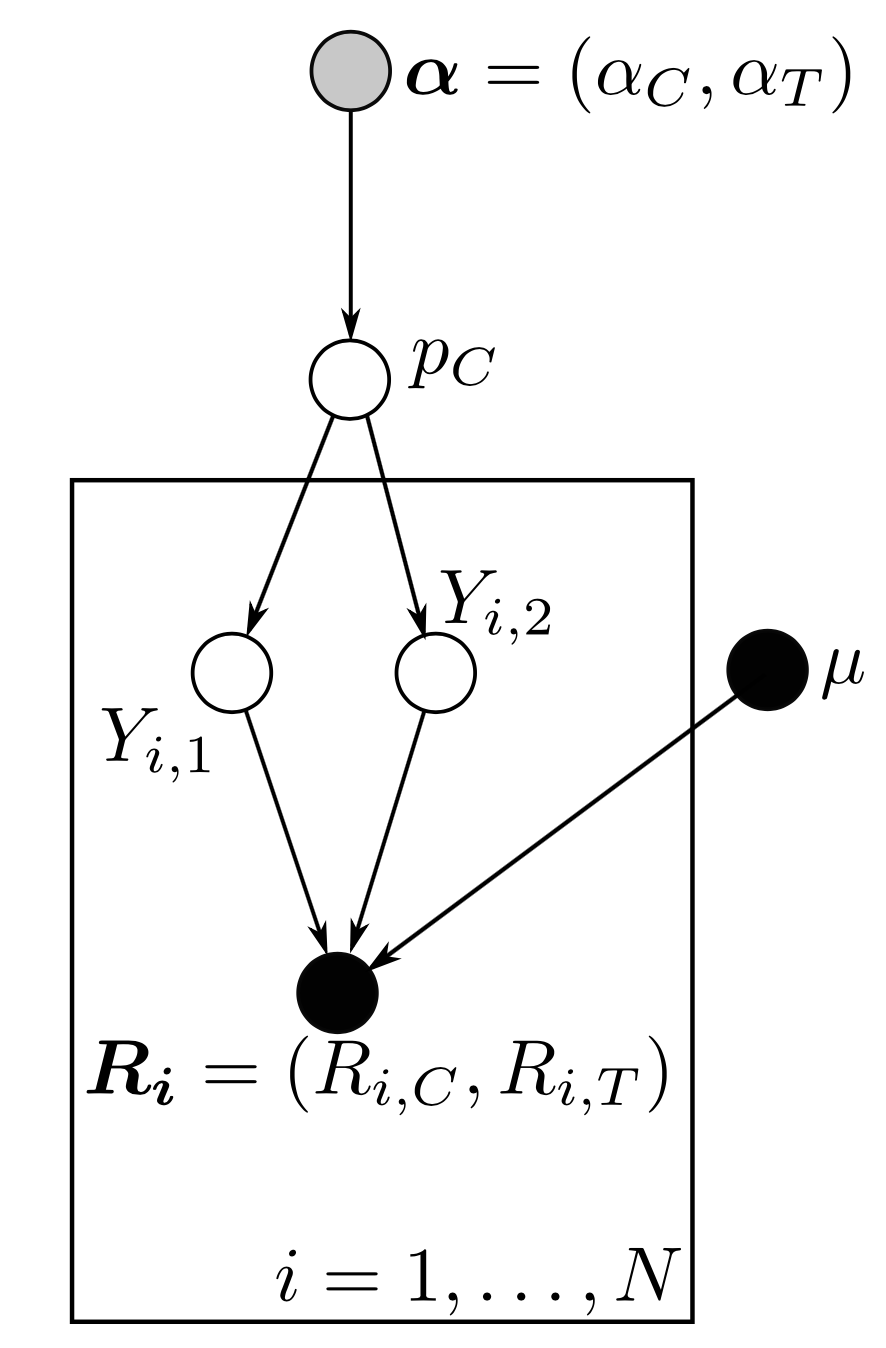
\includegraphics[width=1.0\textwidth]{../diagrams/prob-geno-calling.png}
    \end{column}
    \begin{column}{0.69\textwidth}
    	\begin{itemize}
		\item Gibbs sampling would proceed similarly in this case:
		\begin{itemize}
		\item Start with a guess for $p_C$
		\item Given $p_C$ and the read depths, simulate values for all the $Y_{i,1}$ and $Y_{i,2}$'s
		\item Then, given the $Y_{i,1}$ and $Y_{i,2}$'s, simulate a new $p_C$.
		\end{itemize}
		\item In practice, ANGSD identifies the {\em maximum-a-posteriori} (or MAP) estimate 
		by a related maximization algorithm.
		\item The main point here is that probabilistic genotype calling and allele frequency
		estimation can be done together.
        \end{itemize}
    \end{column}
\end{columns}
\end{frame}








\begin{frame}{INTERMISSION}
\begin{center}
\LARGE Holy Cow! 1 hour 45 minutes is a long session.  Let's take 5 minutes for some
fresh air and then return to assessing errors in RAD-seq data.
\end{center}
\end{frame}











\begin{frame}{RAD-bashing}
\framesubtitle{There have been some criticisms\ldots}
\underline{Allelic dropout / null alleles and other biases}:\\
~~~~~~~~~~~~~~~~~~~~~~~~~~~~~~~~~~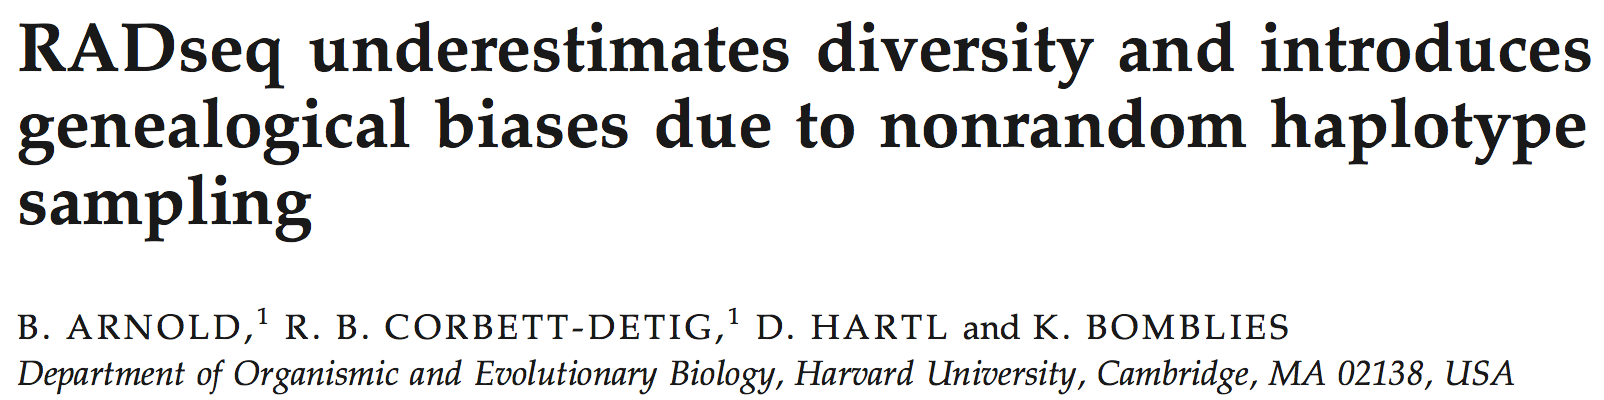
\includegraphics[width=.55\textwidth]{./images/russ.png}\\
~~~~~~~~~~~~~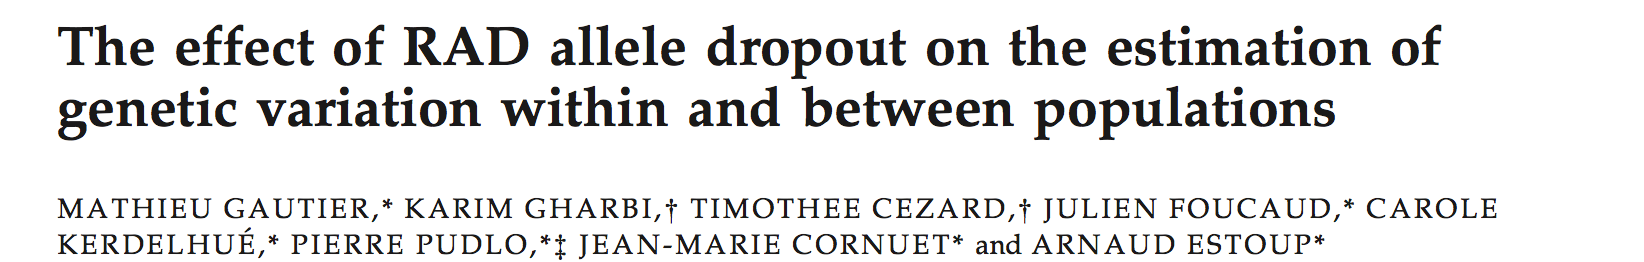
\includegraphics[width=.55\textwidth]{./images/gautier.png}\\
~~~~~~~~~~~~~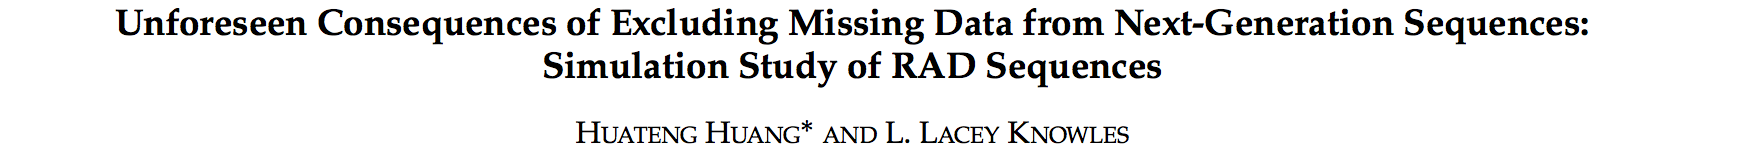
\includegraphics[width=.85\textwidth]{./images/huang.png}\\
\mbox{} \\
\underline{Insufficient genome extent}:\\
~~~~~~~~~~~~~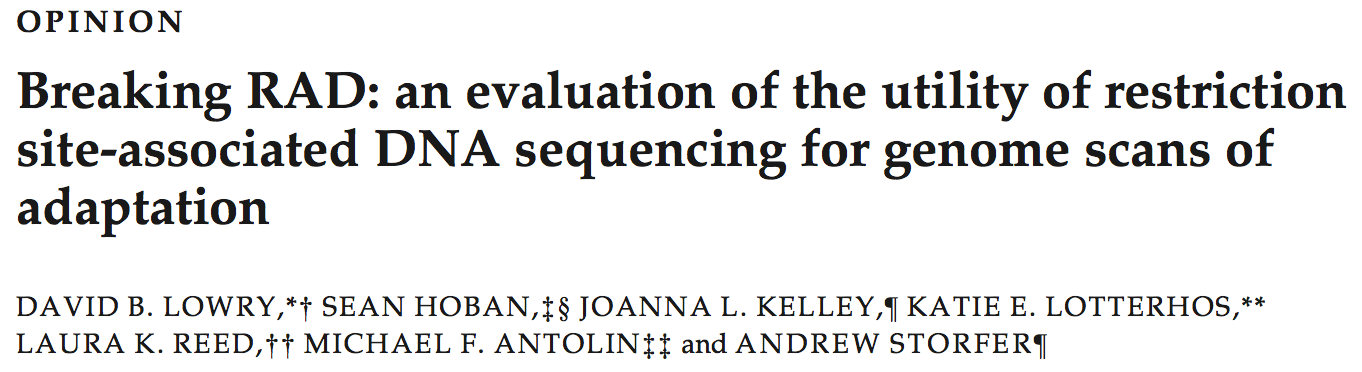
\includegraphics[width=.55\textwidth]{./images/breaking.png}\\

\end{frame}






\begin{frame}{RAD ``Genotyping Accuracy'' Studies}
\framesubtitle{Typically explorations of different bioinformatic settings and filters}
~~~~~~~~~~~~~~~~~~~~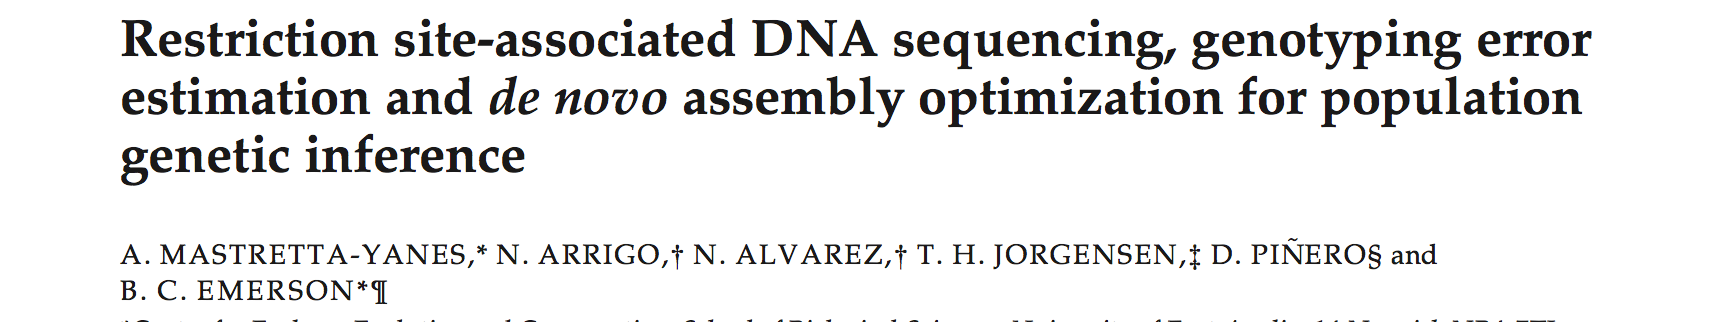
\includegraphics[width=.75\textwidth]{./images/mast.png}\\
\vspace*{1em}
~~~~~~~~~~~~~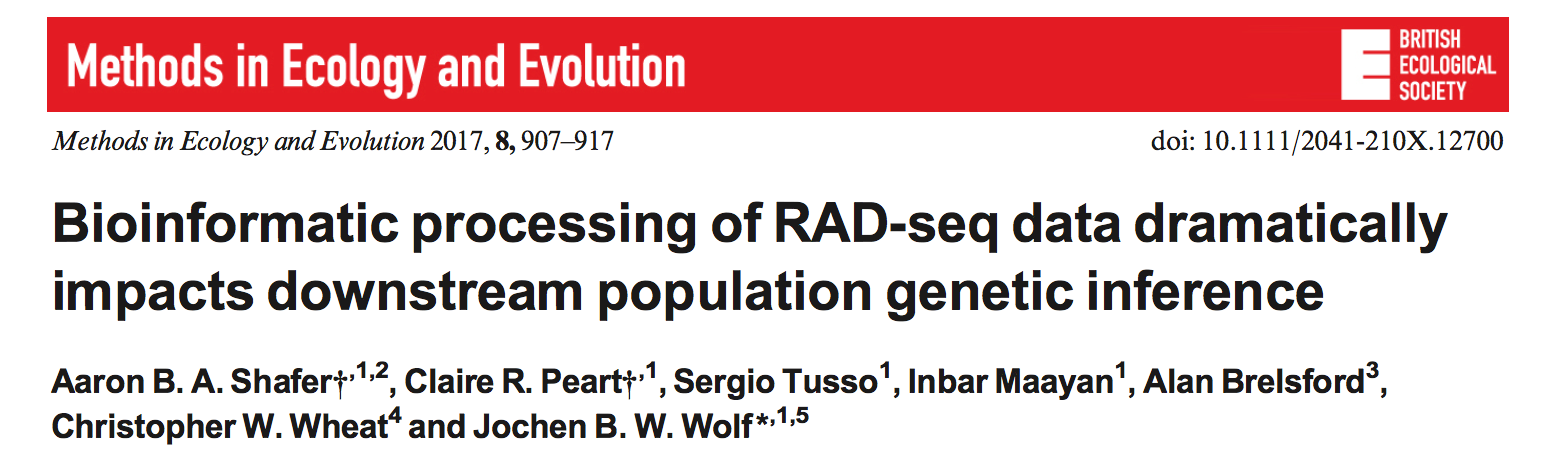
\includegraphics[width=.75\textwidth]{./images/shafer.png}\\
\begin{itemize}
\item Some nice studies
\item A whole lot of computation
\item Not much immediate feedback for individual RAD users or the question of, ``How we doin' here?"
\end{itemize}
\end{frame}








\begin{frame}{A Simple Visualization from Called RAD Genotypes}
\framesubtitle{Some willow flycatcher data I was working with}
Just plot the observed frequency of genotypes against their expected frequency given the allele frequencies and Hardy Weinberg Equilibrium

\begin{center}
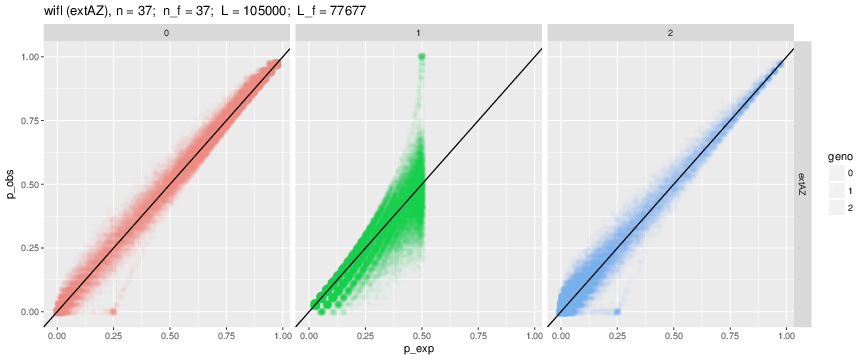
\includegraphics[width=1.0\textwidth]{./images/wifl_big_pop_no_bounds.png}
\end{center}
\end{frame}






\begin{frame}{What Should These Look Like?}
\framesubtitle{Simulate data in perfect HW-equilibrium}

\begin{center}
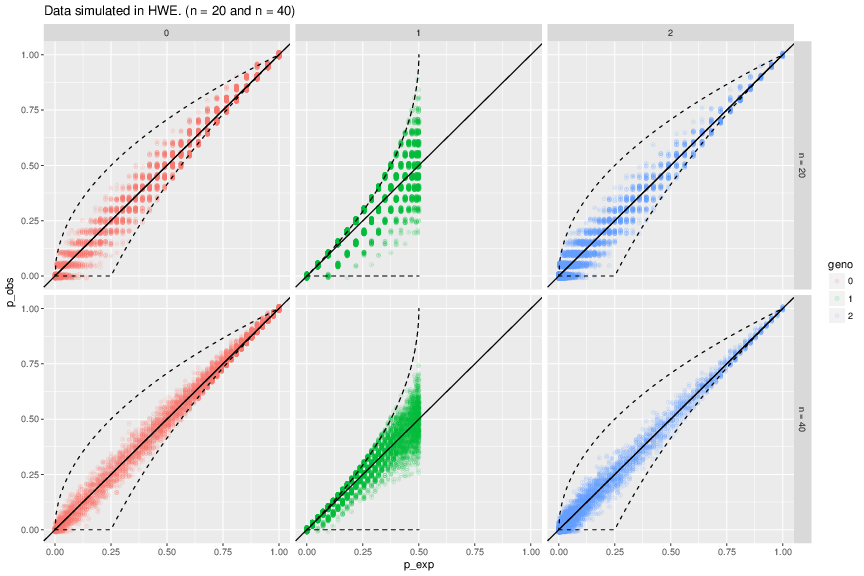
\includegraphics[width=1.0\textwidth]{../figures/simulated-nice-data.png}
\end{center}
\end{frame}







\begin{frame}{Things don't always look so peachy}
\framesubtitle{Published data from lobsters (Benestan et al. 2015)}

This is a sample of individuals that were all collected from the same place that should have been
in HWE\ldots

\begin{center}
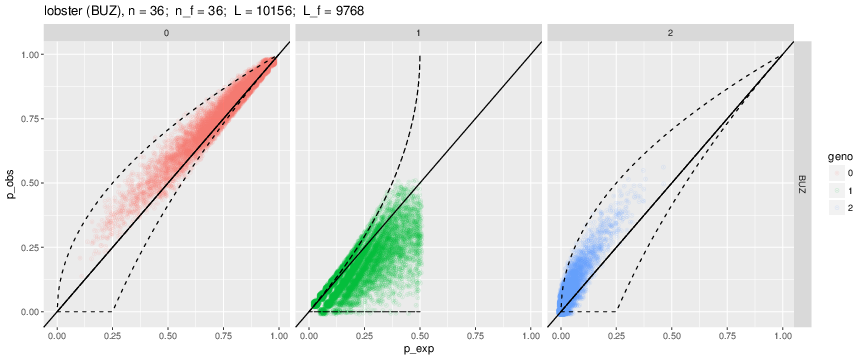
\includegraphics[width=1.0\textwidth]{./images/lobster_big_pop.png}
\end{center}
\end{frame}





\begin{frame}{A Genotyping Error Model}
\framesubtitle{How much error must there be to look that bad?}


\begin{columns}
    \begin{column}{0.38\textwidth}
        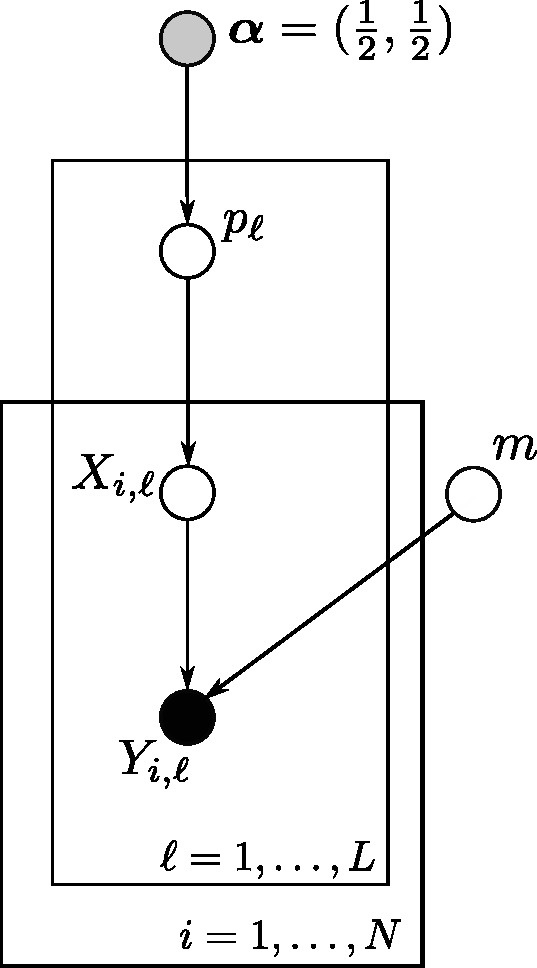
\includegraphics[width=1.0\textwidth]{./images/geno-err-model.pdf}
    \end{column}
    \begin{column}{0.58\textwidth}
        \begin{itemize}
        \item $\bm{\alpha}$~~~~beta prior parameters for allele frequencies
        \item $p_\ell$~~~~unknown frequency of alternate allele at SNP $\ell$
        \item $X_{i,\ell}$~~~~true, underlying, but unobserved, genotype of individual $i$ at SNP $\ell$
        \item $Y_{i,\ell}$~~~~the observed (called/scored) but possibly incorrect genotype of individual $i$ at SNP $\ell$
        \item $m$~~~~the rate at which true heterozygotes are incorrectly called as homozygotes
        \end{itemize}
    \end{column}
\end{columns}
\end{frame}




\begin{frame}{Estimating $m$ via MCMC}
\begin{center}
Willow Flycatchers\\
\vspace*{1em}

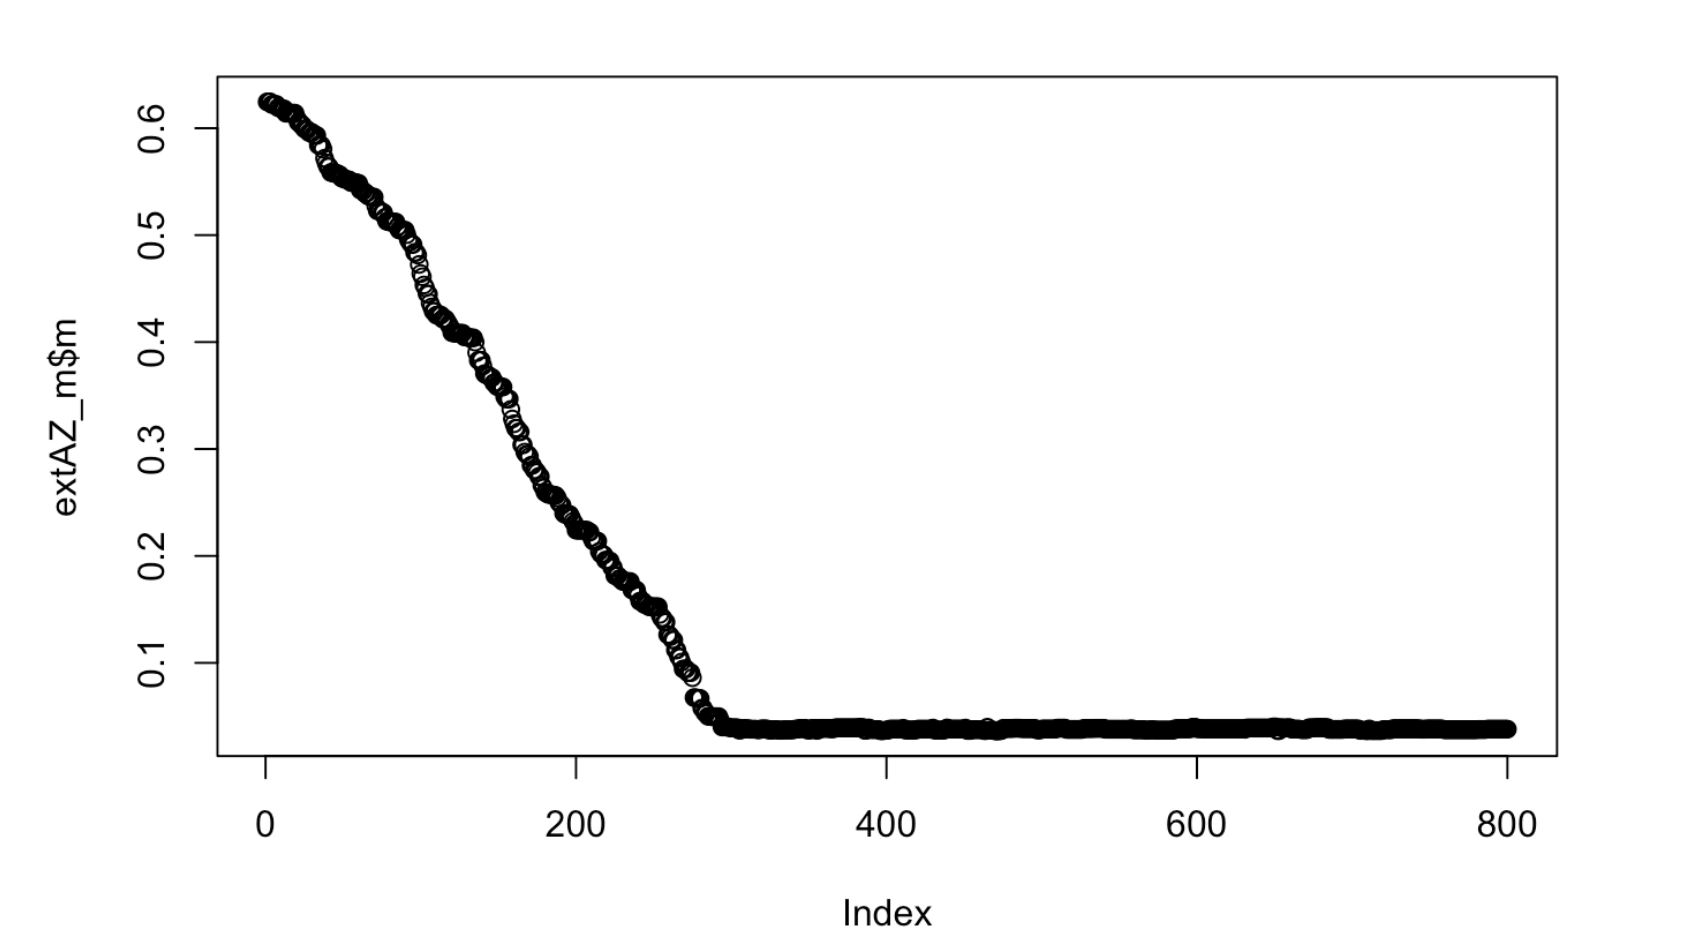
\includegraphics[width=0.87\textwidth]{./images/wifl-trace.png}
\end{center}
\end{frame}




\begin{frame}{Estimating $m$ via MCMC}
\begin{center}
Lobsters\\
\vspace*{1em}

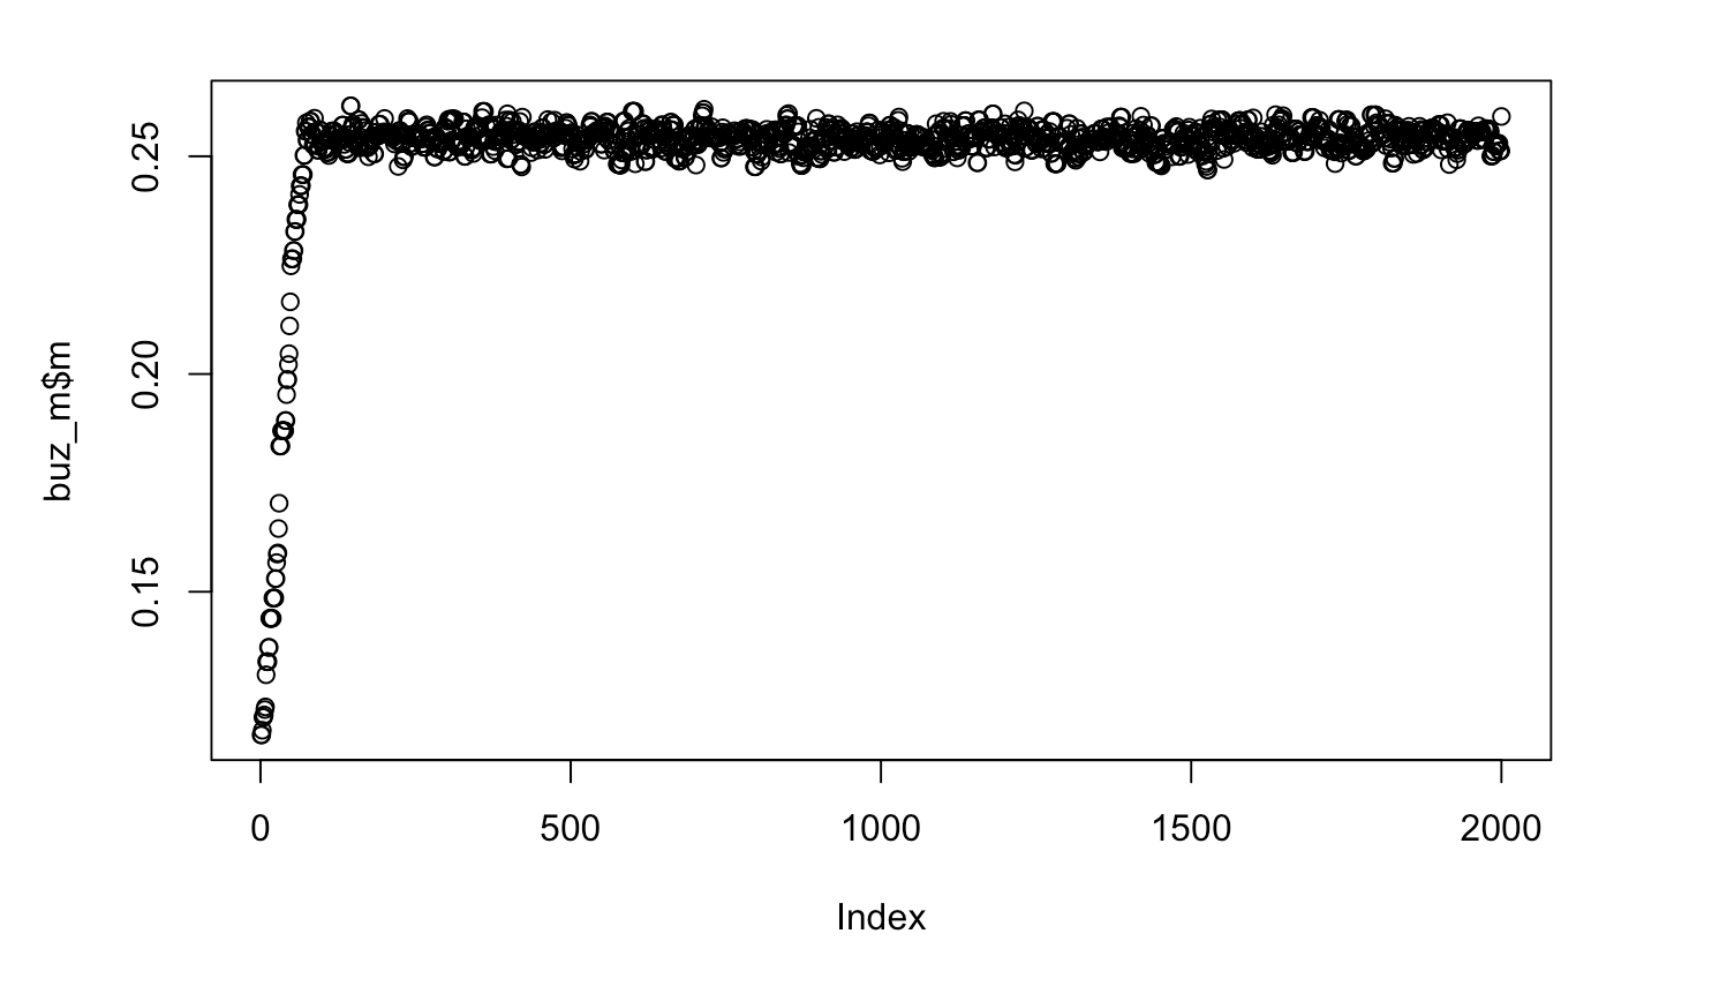
\includegraphics[width=0.87\textwidth]{./images/lobster-trace.png}
\end{center}
Holy Moly!
\end{frame}





\begin{frame}{A Survey of Some Published Data Sets}

\begin{center}
Bonnethead Shark~~~$\hat{m} = 0.01$
\vspace*{1.5em}

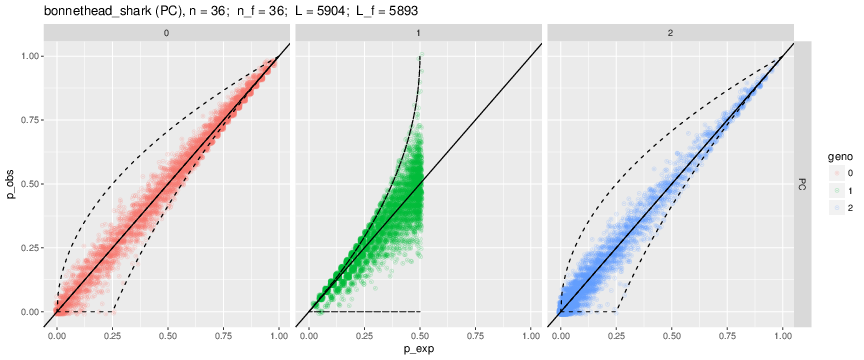
\includegraphics[width=0.87\textwidth]{./images/bonnethead_shark_big_pop.png}
\end{center}
\end{frame}





\begin{frame}{A Survey of Some Published Data Sets}

\begin{center}
Western Alaska Chinook~~~$\hat{m} = 0.02$
\vspace*{1.5em}

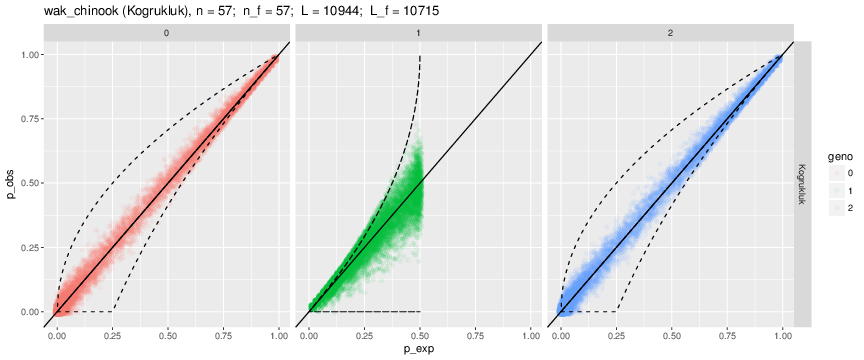
\includegraphics[width=0.87\textwidth]{./images/wak_chinook_big_pop.png}
\end{center}
\end{frame}





\begin{frame}{A Survey of Some Published Data Sets}

\begin{center}
Red Drum~~~$\hat{m} = 0.05$
\vspace*{1.5em}

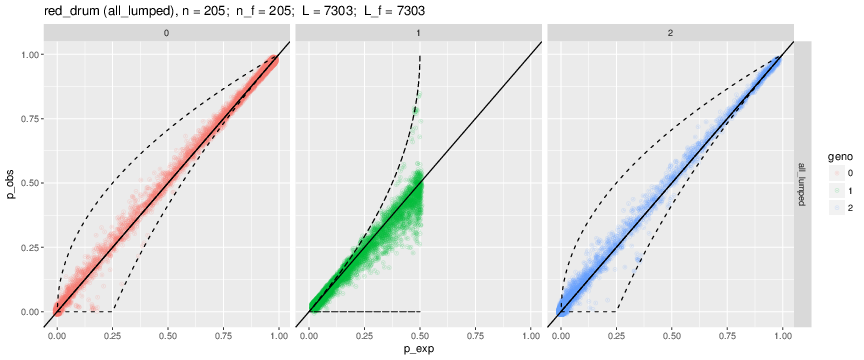
\includegraphics[width=0.87\textwidth]{./images/red_drum_big_pop.png}
\end{center}
\end{frame}






\begin{frame}{A Survey of Some Published Data Sets}

\begin{center}
Anguilla~~~$\hat{m} = 0.14$
\vspace*{1.5em}

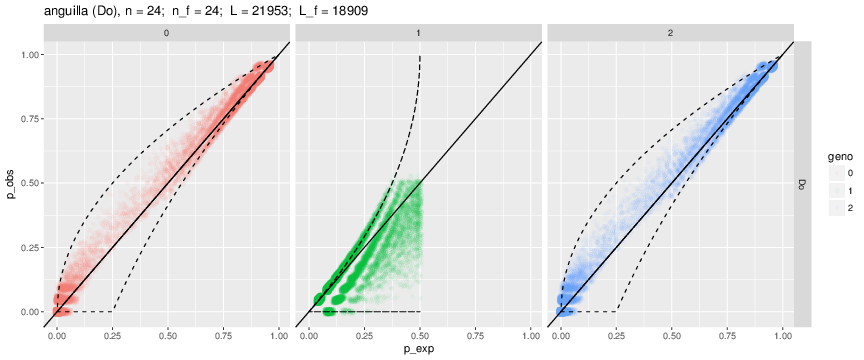
\includegraphics[width=0.87\textwidth]{./images/anguilla_big_pop.png}
\end{center}
\end{frame}






\begin{frame}{A Survey of Some Published Data Sets}

\begin{center}
Columbia River Chinook~~~$\hat{m} = 0.17$
\vspace*{1.5em}

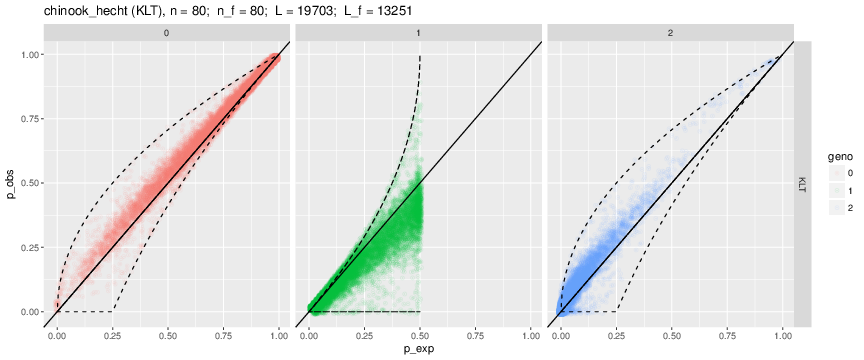
\includegraphics[width=0.87\textwidth]{./images/chinook_hecht_big_pop.png}
\end{center}
\end{frame}




\begin{frame}{A Survey of Some Published Data Sets}

\begin{center}
Anchovy~~~$\hat{m} = 0.28$
\vspace*{1.5em}

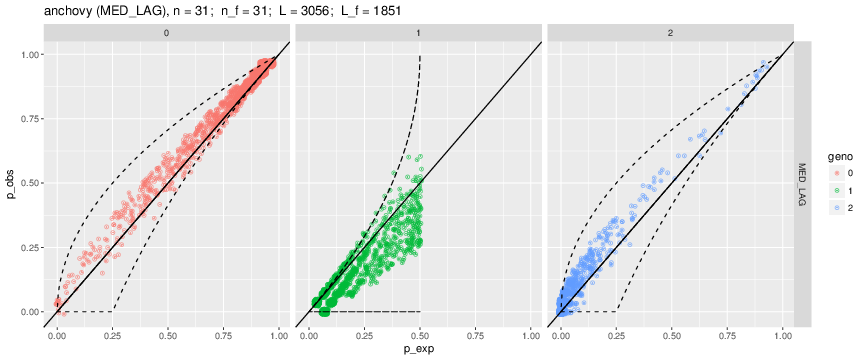
\includegraphics[width=0.87\textwidth]{./images/anchovy_big_pop.png}
\end{center}
\end{frame}




\begin{frame}{A Survey of Some Published Data Sets}

\begin{center}
Snails~~~$\hat{m} = 0.45$
\vspace*{1.5em}

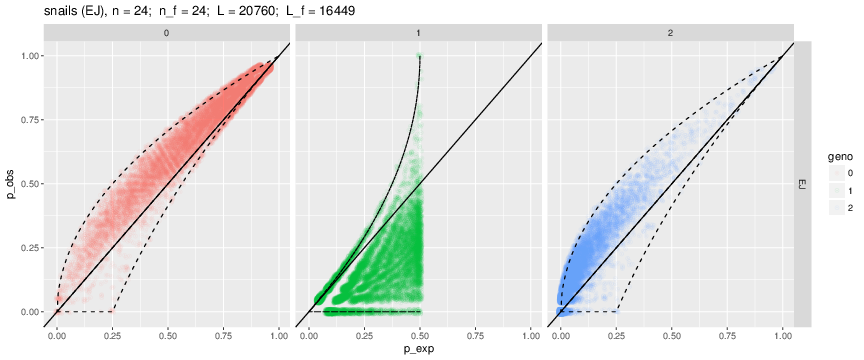
\includegraphics[width=0.87\textwidth]{./images/snails_big_pop.png}
\end{center}
\end{frame}



\begin{frame}{A Survey of Some Published Data Sets}

\begin{center}
Dolphin~~~$\hat{m} = 0.72$
\vspace*{1.5em}

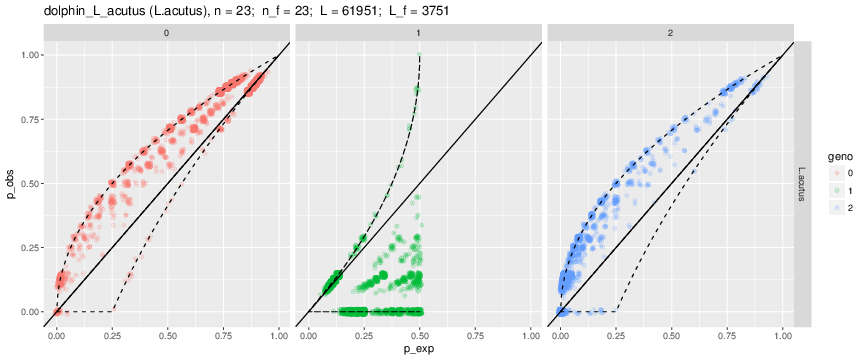
\includegraphics[width=0.87\textwidth]{./images/dolphin_L_acutus_big_pop.png}
\end{center}
\end{frame}





\begin{frame}{Include Read Depth in the Genotyping Error Model}
\framesubtitle{Is this error mostly a consequence of inaccuracy at low read depths?}


\begin{columns}
    \begin{column}{0.38\textwidth}
        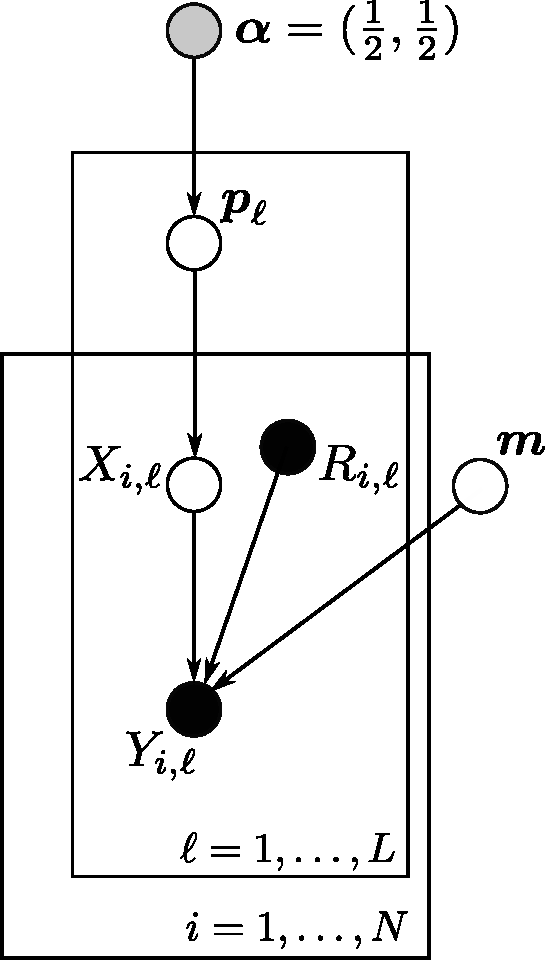
\includegraphics[width=1.0\textwidth]{./images/geno-err-model-with-read-depth.pdf}
    \end{column}
    \begin{column}{0.58\textwidth}
        \begin{itemize}
        \item $R_{i,\ell}$ the read-depth category or bin of the $\ell\thh$ SNP in the $i\thh$ individual.
        \item $\bm{m}$~~~~This is now a vector---a separate heterozygote miscall rate for each read depth category.
        \end{itemize}
    \end{column}
\end{columns}
\end{frame}






\begin{frame}{Het Miscall Rate Higher at Low Read Depth}

\begin{center}
Lobster~~~overall $\hat{m} = 0.25$
\vspace*{1.5em}

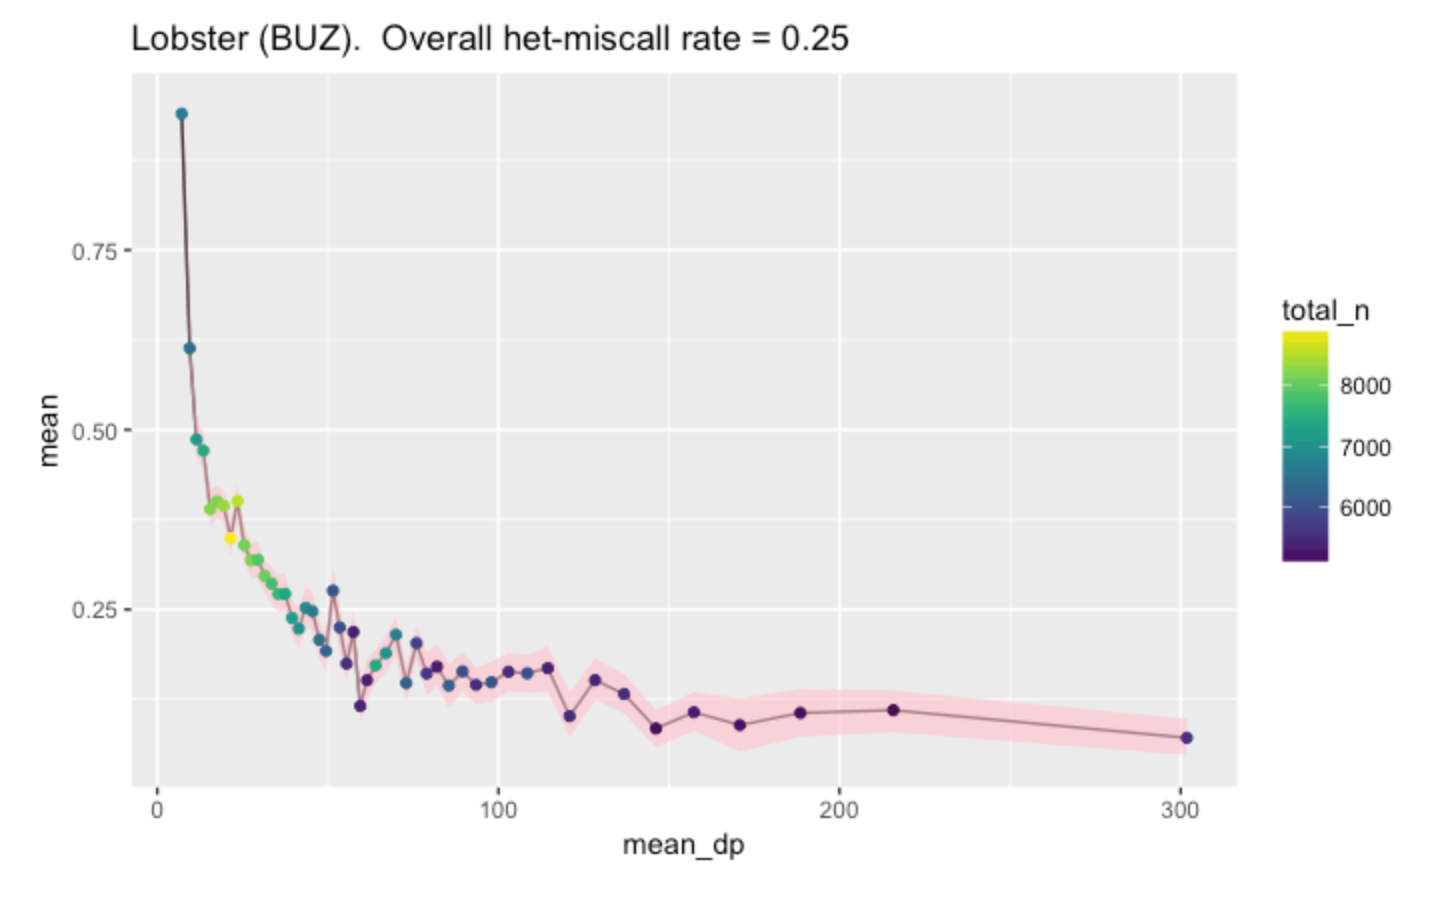
\includegraphics[width=0.87\textwidth]{./images/lobster-dp.png}
\end{center}
\end{frame}




\begin{frame}{This Trend Seen Even in ``High Accuracy'' Data Sets}

\begin{center}
Bonnethead Shark~~~overall $\hat{m} = 0.01$
\vspace*{1.5em}

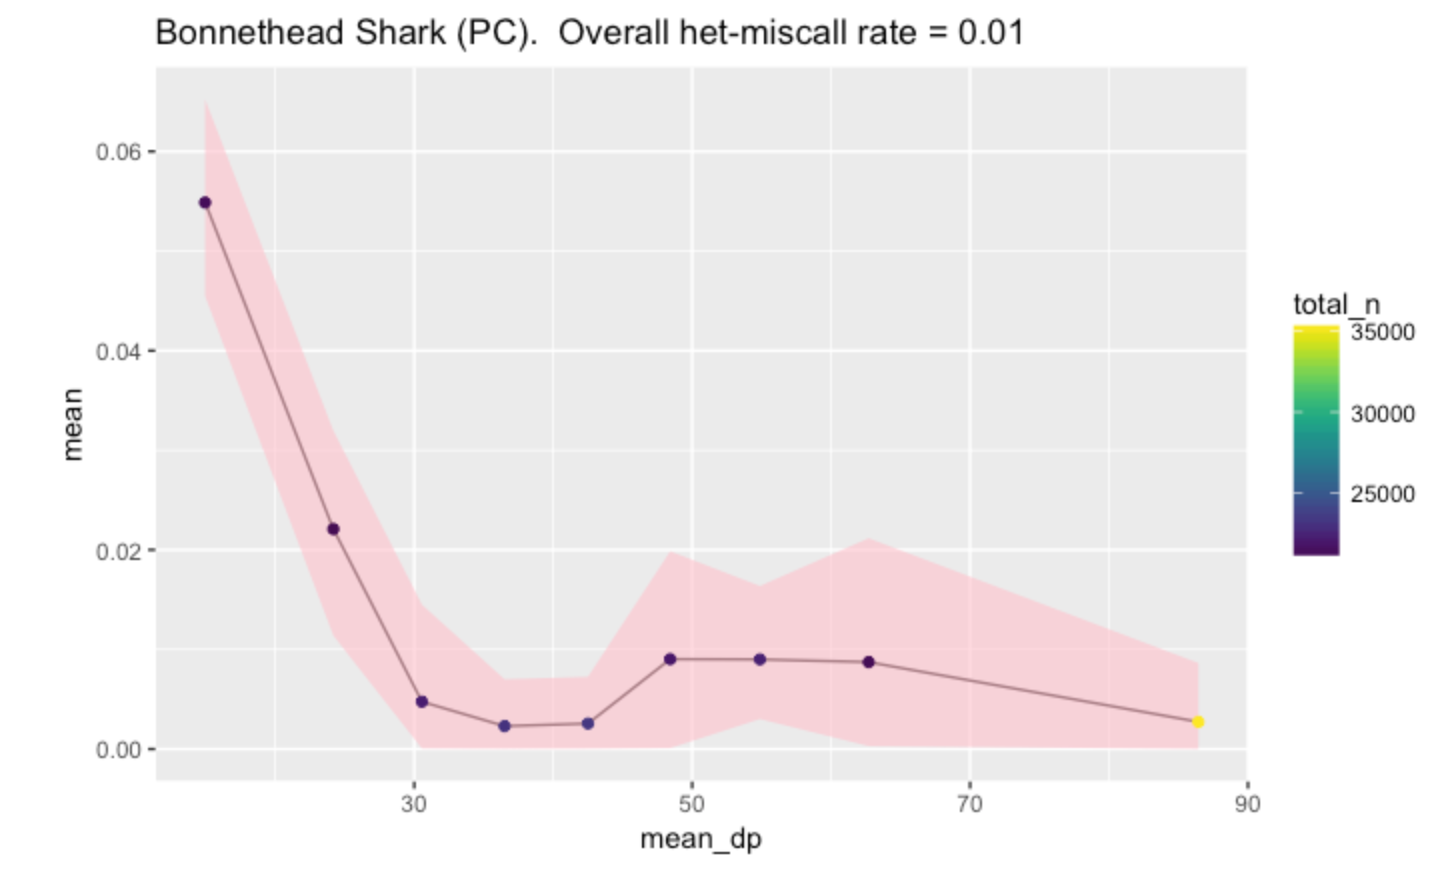
\includegraphics[width=0.87\textwidth]{./images/bonnethead-shark-dp.png}
\end{center}
\end{frame}




\begin{frame}{This Trend Seen Even in ``High Accuracy'' Data Sets}

\begin{center}
Red Drum~~~overall $\hat{m} = 0.05$
\vspace*{1.5em}

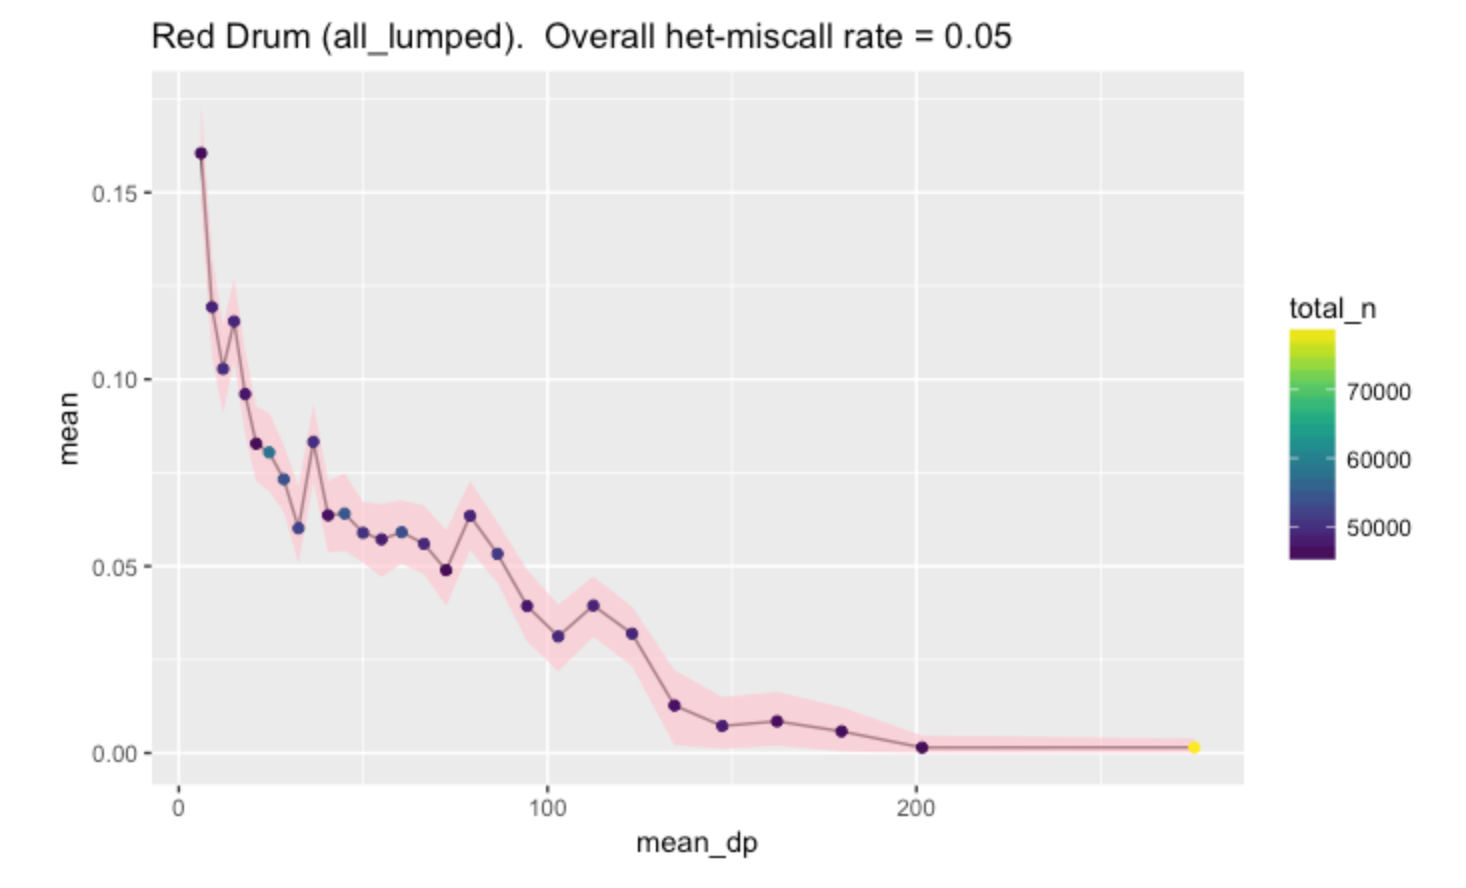
\includegraphics[width=0.87\textwidth]{./images/red-drum-dp.png}
\end{center}
\end{frame}




\begin{frame}{Wrap Up}
\begin{itemize}
\item Working on a paper with Gordon Luikart and Thierry Gosselin doing a 
more complete survey.  
\item While RAD suffers some known biases, there are also problems
with straight-up genotyping error.
\item A primary driver seems to be insufficient read depth to call heterozygotes
\item Effects on downstream analysis depend on what you are doing:
\begin{itemize}
\item Allele frequency estimation (not too bad)
\item Relationship inference (disastrous)
\item Identification of $F_{ST}$ outliers (potentially problematic)
\item etc.
\end{itemize}
\item All this would benefit from a probabilistic genotype calling approach, incorporating a prior on 
genotype frequencies
\end{itemize}
\end{frame}




\begin{frame}{Hands-On Session.  Using R package {\tt whoa}}
\begin{itemize}
\item {\tt whoa} is available on GitHub (would have been on CRAN, but they CRANsters were on vacation last week!  :-(~~)
\item I have made precompiled binaries for Mac and Windows.
\item I've prepared a simple R notebook for installation and the hands-on exercises. Find that at:
 \url{https://eriqande.github.io/con-gen-2018/whoa\_hands\_on.nb.html}
\end{itemize}
\end{frame}



\end{document}



